\documentclass[a4paper,12pt]{report}
\usepackage[utf8]{inputenc}
\usepackage[russian]{babel}
\setlength{\parskip}{0ex}
\usepackage{indentfirst}
\usepackage{xcolor}
\usepackage{hyperref}
\usepackage{verbatim}
\usepackage{natbib}
\usepackage{graphicx}
\usepackage{titlesec}
\usepackage[nottoc,numbib]{tocbibind}
\titleformat{\chapter}
       {\normalfont\fontsize{16pt}{16}\bfseries}{\thechapter}{1em}{}
\titleformat{\section}
       {\normalfont\fontsize{14pt}{14}\bfseries}{\thesection}{1em}{}
\titleformat{\subsection}
       {\normalfont\fontsize{12pt}{12}\bfseries}{\thesubsection}{1em}{}
\titlespacing*{\chapter}{0pt}{0pt}{16pt}
\usepackage[a4paper,left=3cm,right=1.5cm,top=2cm,bottom=2cm]{geometry}
\setlength{\parindent}{1.25cm}
\renewcommand{\baselinestretch}{1.5}

\makeatletter
\newcommand*{\centerfloat}{%
  \parindent \z@
  \leftskip \z@ \@plus 1fil \@minus \textwidth
  \rightskip\leftskip
  \parfillskip \z@skip}
\makeatother

\title{Алгоритмы, используемые в компьютерных играх}
\author{Рахимянов Э. Ш.}
\date{Июнь, 2019г.}

\begin{document}

\maketitle

\begin{abstract}
Дипломная работа содержит пояснительную записку,
изложенную на 31 страницах печатного текста, содержит 16 изображений и 1 таблицу.

\textit{\textbf{Ключевые слова --- }алгоритмы, игры, упаковка в контейнер, процедурная генерация, пикселизация.}

Объектом исследования являются некоторые алгоритмы, применяющиеся в компьютерных играх.

Цель работы – выявление новых и анализ существующих алгоритмов упаковки в контейнер, процедурной генерации уровня и пикселизации.

Результатом работы стала реализация данных методов на стеке технологий\newline HTML/CSS/JS.

В работе предложено описание и сравнение разных алгоритмов. Разработаны графические приложения и библиотеки для решения данных проблем; исходный код и демонстрационные варианты доступны в Интернете. В дальнейшем их можно использовать для создания собственной игры или исследовании новых алгоритмов.
\end{abstract}

\tableofcontents

\chapter{Вступление}

\parindent=1cm
Игровая индустрия значительно преобразилась в последние годы. Согласно опросу Entertainment Software Association, количество американцев, играющих в видеоигры выросла с 59\% в 2014 до 65\% в 2019; 46\% из них женщины, общий средний возраст игроков - 33 года \citep{esa_old}\citep{esa}.

В начале 2019 года я с моим приятелем загорелись желанием сделать компьютерную игру своей мечты. К сожалению для нас, эта затея оказалась не такой простой для воплощения в жизнь по причине возникновения многих проблем. Некоторые из них решены алгоритмически и будут подробно описаны далее. Давайте кратко рассмотрим их.

\section{Формирование текстурного атласа}

Текстурный атлас - это изображение, в котором расположены все игровые текстуры без повторений так, что они попарно не пересекаются. Атлас нужен для быстрой отрисовки текстур в реальном времени и используется в подавляющем большинстве компьютерных игр (например, в игровом движке Unity\citep{unity}). Данная проблема имеет модель задачи об упаковке прямоугольников в контейнеры.

\section{Создание игровых уровней}

Поскольку жанром нашей игры стал \textit{roguelike}, а по канону этого жанра уровни генерируются случайным образом, необходимо было придумать, как создавать уровни, которые будут интересны для будущих игроков. Динамический метод создания игровых карт используется, например в крупной франшизе пошаговых игр Civilization\citep{civi}.

\section{Создание игровых спрайтов}

Чтобы нарисовать спрайты персонажей и окружения для игры, требуется большое количество времени и опыта в соответствующей сфере, которых у нас не было. Поэтому было принято решение о стилизации спрайтов, находящихся в открытом доступе. Стилем был выбран пиксель-арт, который применялся в крупной франшизе игр Sonic the Hedgehog\citep{sonic}.

\chapter{Задача об упаковке в контейнер} 

\parindent=1cm
Задача об упаковке в контейнеры \citep{Jylanki} двумерных прямоугольников это классическая проблема комбинаторных оптимизаций. Она заключается в том, что дана последовательность прямоугольников $(R_1, R_2, …, R_n), R_i = (w_i, h_i)$ и нужно найти упаковку этих элементов в минимальное количество контейнеров размера $(W, H)$. Ни один из двух прямоугольников не может пересекаться или располагаться один в другом. Задача имеет несколько реализаций, и её NP-трудность доказывается сведением к задаче разбиения множества чисел. Задача не решается за полиномиальное время, но имеет полиномиальную сложность. В основном оптимальное решение достигается за счёт эвристических алгоритмов.

Задача двумерной контейнерной упаковки это обобщение одномерной задачи контейнерной упаковки. Существуют два варианта двумерной задачи. В первом процесс моделируются так, что прямоугольники получены из некоторых входных данных за раз, а потом они должны немедленно разместиться в один из контейнеров, ничего не зная о последующих элементах. Этот вариант — \textit{онлайн} упаковка прямоугольников в контейнеры. Второй вариант — это \textit{офлайн} упаковка прямоугольников в контейнеры, в котором вся последовательность для упаковывания известна заранее. Рассмотрим алгоритмы обоих вариантов.

В первой формулировке задачи об упаковке в контейнеры может существовать несколько одновременно \textit{открытых} контейнеров, между которыми  алгоритм может выбрать место назначения для текущего прямоугольника. В более строгом варианте есть ограничение на количество контейнеров, которые могут быть открыты в одно время , и для того, чтобы открыть новый, существующий контейнер должен быть \textit{закрыт}. Алгоритмы семейства -BNF могут быть использованы для самого строгого случая, где открыт только один контейнер за раз; другие семейства покрывают случаи, когда нет ограничений на число открытых контейнеров.

Способ упаковки называется \textit{ортогональным}, если стороны размещенных прямоугольников параллельны ребрам контейнера. Предположим, что упаковки ортогональны и каждый прямоугольник может быть повернут на 90 градусов. Такой способ упаковки называется \textit{поворотным} и позволяет выбрать на вход $R = (w, h)$ или $R’ = (h, w)$.

В некоторых прикладных реализациях требуется, чтобы процесс упаковки был \textit{гильотинированным}. Упаковка $P$ гильотинирована, если ее можно разделить на две части $P_1$ и $P_2$ одним прямым горизонтальным или вертикальным разрезом, который не пересекает ни один из прямоугольников в упаковке, и где оба $P_1$ и $P_2$ гильотинированы или каждый вмещает по одиночному прямоугольнику.

Алгоритмы, реализующие задачу об упаковке в контейнеры, классифицируются по группам в зависимости от используемой структуры данных  и свободного места, оставшегося в контейнере. Начнем с самого простого и продолжим наиболее сложными.

\section{Алгоритмы выступа (shelf algorithms)}

Алгоритмы выступа (или алгоритмы уровня) используют самые простые методы для упаковывания. Будем считать, что \textit{выступ} — это внутренний прямоугольник контейнера с шириной $W_b$ и и высотой $h_s$. Когда начинается упаковывание, свободное пространство контейнера преобразовывается в выступы, располагающиеся снизу вверх, в которых прямоугольники размещены слева направо. Последний выступ (выступ на вершине) называется \textit{открытым}. Из-за того, что прямоугольники размещаются снизу вверх, пространство над открытым выступом не используется. Благодаря этому высота открытого выступа может быть вычислена в любое время, когда прямоугольник находится на этом выступе. Для выступов, которые находятся под открытым, нет таких возможностей, поэтому их называют \textit{закрытыми}.

При упаковке прямоугольника $(w, h)$ в выступ $(W_b, h_s)$ нужно выбрать, поворачивать прямоугольник или нет, то есть, будет ли он храниться вертикально  $(min(w, h), max(w, h))$ или горизонтально $(max(w, h), min(w, h))$. При любой реализации действовать следующим образом:

1. Если прямоугольник является первым на новом открытом выступе, то он хранится горизонтально. Так минимизируется высота нового выступа.

2. Если прямоугольник выровнен вертикально (например, $max(w, h) < h_s$), то так его и храним. Это минимизирует потерянное пространство между верхней стороной прямоугольника и верхней линией выступа.

3. В любом другом случае лучше хранить прямоугольник горизонтально.

\begin{figure}
    \centerfloat
    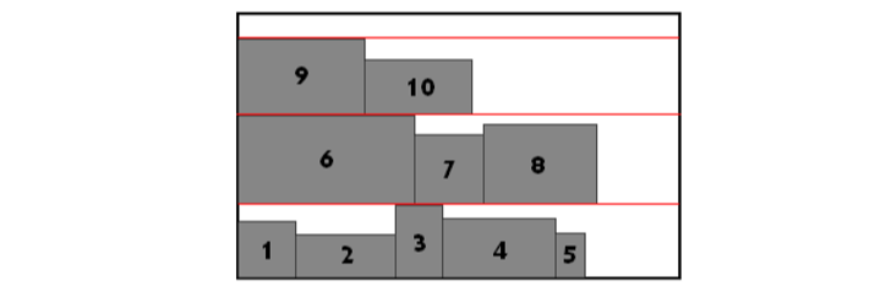
\includegraphics[width=1\textwidth]{packing/1.png}
    \caption{Пример упаковки алгоритмом выступа}
    \label{fig:shelf}
\end{figure}

На рис. \ref{fig:shelf} показан пример упаковки в контейнеры с помощью алгоритма выступа. Прямоугольники пронумерованы в порядке следования в контейнере, а красная линия показывает верхнюю линию выступа. Все варианты алгоритма выступа производят упаковку, очень похожую на ту, что на картинке.

Алгоритм выступа подходящего следующего (shelf next fit, shelf-NF) очень прост, потому что его сложность $O(1)$ по памяти и $\theta(n)$ по времени. Этот алгоритм далеко не лучший из всех. Для каждого прямоугольника определяем его ориентацию. Пытаемся поставить прямоугольник в текущий открытый выступ. Если прямоугольник не влезает, закрываем текущий выступ и открываем новый. Если выступов не осталось, завершаем.

Алгоритм выступ первого подходящего (shelf first fit, shelf-ff) реализуется за $O(nlogn)$ по времени и $O(n)$ по памяти. Чтобы не забывать о свободном месте в старых закрытых выступах, нужно поддерживать список закрытых выступов. Если оказалось несколько закрытых выступов, куда может влезть прямоугольник, то следует выбрать тот, у которого наименьший индекс.

Алгоритм лучшего выступа по ширине (shelf best width fit, shelf-bwf) из всех закрытых выступов выбирает тот, у которого ширина свободного места выступа минимальна.

Алгоритм лучшего выступа по высоте (shelf best height fit, shelf-bhf) решает проблему прямоугольников, которые по высоте ниже верхней линии выступа. Алгоритм выбирает выступы с минимальной оставшейся высотой $hs - h$.

Алгоритм лучшего выступа по свободной области (shelf best area fit, shelf-baf) комбинирует два предыдущих, выбирая тот выступ, у которого оптимально можно использовать и ширину и высоту.

Алгоритм худшего выступа по ширине (shelf worst width fit, shelf-wwf) является полной противоположностью shelf-bwf, так как оставляет каждый выступ с максимально возможной шириной. Хотя shelf-wwf и shelf-bwf делают противоположные вещи, невозможно определить, какой из них эффективнее.

Сложность всех алгоритмов выше $O(n^2)$ по времени и $O(n)$ по памяти.

Зато алгоритм верхней линии выступа (shelf floor-ceiling) избавлен от проблемы, когда нельзя вернуть область у прямоугольников, чья высота не соответствует высоте выступа. Прямоугольники сортируются по убыванию размера длинной стороны и упаковываются слева направо.

\section{Алгоритмы гильотины (guillotine algorithms)}

Какие уловки ни используй для улучшения алгоритмов выступа, всё равно в худшем случае потеряется много места. Алгоритмы гильотины базируются на размещении гильотинного разрыва — операции, которая помещает прямоугольник в свободный угол контейнера, после чего оставшаяся $L$-область контейнера делится на ещё два непересекающихся прямоугольника. (рис. \ref{fig:guil})

\begin{figure}
    \centerfloat
    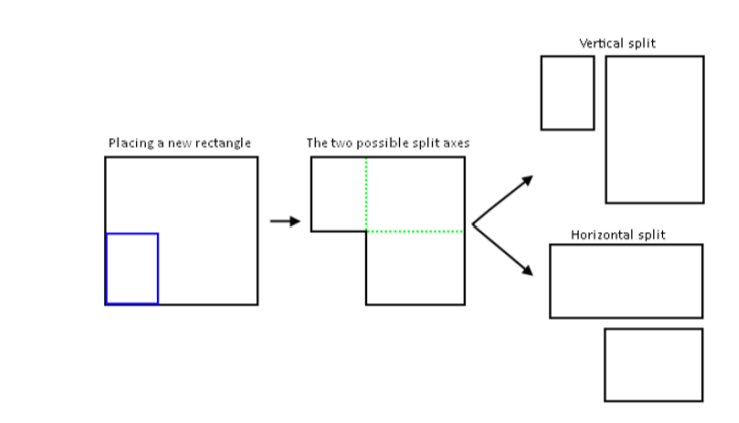
\includegraphics[width=0.8\textwidth]{packing/2.png}
    \caption{Базовый принцип алгоритмов гильотины \citep{Jylanki}}
    \label{fig:guil}
\end{figure}

Алгоритмы с подобным разделением находят широкое применение. Однако непонятно, кто первым додумался применять этот алгоритм, поэтому он называется просто гильотинным.

Гильотинные алгоритмы работают следующим образом. Мы имеем список прямоугольников $S = {F_1, … , F_n}$, который отображается в свободное пространство контейнера. Прямоугольники попарно не пересекаются, т. е. $F_i \cap F_j =$ $\O$ для всех $i \neq j$ и общая неиспользуемая свободная область контейнера равная объединения прямоугольников $(\cupF_i)$. Алгоритм начинает c одного прямоугольника $S = {F_1 = (W, H)}$. На каждом шаге упаковки мы вначале берем свободный прямоугольник $F_i$, а внутри него размещаем следующий прямоугольник $R = (w, h)$ в нижнем левом углу. Оставшееся место в $F_i$ гильотинируется на два меньших прямоугольника $F’$ и $F’’$, которые замещают $F_i$ в списке свободных прямоугольников. Процедура продолжается, пока не останется свободных прямоугольников, которые могут вместить  себя следующий за ними, и начинается снова на новом пустом контейнере.

\begin{figure}
    \centerfloat
    
\includegraphics[width=1.5\textwidth]{packing/3.png}
    \caption{Пример упаковки алгоритмом гильотины \citep{Jylanki}}
    \label{fig:guil2}
\end{figure}

Недостаток алгоритма гильотины в том, что он выполняет размещение только если прямоугольник R полностью вмещается в $F_i$. Он никогда не пытается упаковать R на позицию, где гильотинный разрыв накроется прямоугольником.

Алгоритм дополняют два правила. Первое: нужно придумать, как выбрать $F_i$. Второе: нужно выбрать, в каком из двух направлений будет производиться гильотинный разрыв. Различные алгоритмы будут появляться из комбинации этих двух правил.

Алгоритм гильотины по лучшей свободной области (Guillotine Best Area Fit\newline (GUILLOTINE-BAF)) очень похож на shelf-baf тем, что берется свободный прямоугольник $F_i$ минимальной площади, в которую влезет следующий прямоугольник. Это естественное правило, позволяющее узкие полоски неиспользуемого пространства.

Алгоритм гильотины по лучшей меньшей стороне (Guillotine Best Short Side Fit (GUILLOTINE-BSSF)) состоит в том, что когда мы помещаем $R = (w, h)$ в $F_i = (w_i, f_i)$, мы рассматриваем разницу в длине сторон прямоугольников. Алгоритм упаковывает $R$ в такой $F_i$, что $min(w_f - w, h_f - h)$ наименьший. Минимизируется длина меньшей стороны прямоугольника.

Алгоритм гильотины по лучшей большей стороне (Guillotine Best Long Side Fit (GUILLOTINE-BLSF)) действует как предыдущий, только выбирает прямоугольники так, что $max(w_f - w, h_f — h)$ наименьший. Минимизируется длина большей стороны прямоугольника.

Алгоритмы гильотины с плохими правилами вхождения (Guillotine Worst Fit Rules) содержат в себе:
1. Алгоритм гильотины по худшей свободной области (Guillotine Worst Area Fit (GUILLOTINE-WAF)), который аналогичен GUILLOTINE-BAF, только берется $F_i$ максимальной площади
2. Алгоритм гильотины по худшей меньшей стороне (Guillotine Worst Short Side Fit (GUILLOTINE-WSSF)), который аналогичен GUILLOTINE-BSSF, только длина меньшей стороны прямоугольника  максимизируется
3. Алгоритм гильотины по худшей большей стороне (Guillotine Worst Long Side Fit (GUILLOTINE-WLSF)), который аналогичен GUILLOTINE-BLSF, только длина большей стороны прямоугольника максимизируется.

Все эти алгоритмы работают за $O(n^2)$ по времени и $O(n)$ по памяти.

Алгоритм Rectangle Merge Improvement (-RM) после упаковки прямоугольника просматривает все свободные прямоугольники, ища пару соседей $F_i$ и $F_j$ таких, что их объединение может быть представлено одним большим прямоугольником. Если такие есть, они сливаются в один, что эффективно убирает гильотинный разрыв, который образовался бы между $F_i$ и $F_j$. Этот алгоритм сработает за $O(n^3)$ по времени и $O(n)$ по памяти. 

\subsection{Выбор разрыва для алгоритмов гильотины}

Так как разрыв определяет размер свободных прямоугольников и место положение прямоугольника не всегда накрывает линию разрыва, очень важно как именно происходит разрыв, а именно горизонтально или вертикально. Прямоугольник $F_i = (w_f, h_f)$, а внутри него упакован прямоугольник $R = (w, h)$.

Выбор направления разрыва выполняется за константу, поэтому не увеличивает сложность основного алгоритма. 

Правило длинной/короткой оси (Shorter/Longer Axis Split Rule (-SAS, -LAS)) — в случае короткой оси делаем разрыв горизонтальным, если $w_f < h_f$, а иначе делаем разрыв вертикальным. В случае длинной оси делим горизонтально, если $w_f >= h_f$, а иначе вертикально.

Правило длинной/короткой оставшейся оси (Shorter/Longer Leftover Axis Split Rule (-SLAS, -LLAS)) проверяет оставшиеся длины $w_f – w$ и $h_f – h$ прямоугольника. В случае короткой оси делим горизонтально, если $w_f - w < h_f – h$, иначе вертикально. В случае длинной оси делим горизонтально, если  $w_f - w >= h_f – h$, иначе вертикально.


\section{Алгоритмы максимальных прямоугольников}

Алгоритмы гильотины работают гораздо лучше алгоритмов выступа, но ограничения, вызванные линией разрыва, все равно вызывают проблемы. Их решает алгоритм максимальных прямоугольников. Алгоритм базируется на расширении правила размещения гильотинного разрыва. Алгоритм максимальных прямоугольников тоже хранит список свободных прямоугольников, который отображается в пространство контейнера. Однако в отличии от гильотинного алгоритма, который выбирает один из двух направлений разрыва, алгоритм максимальных прямоугольников проводит сразу две оси разрыва.

Процесс разрыва происходит следующим образом. Когда мы ставим входной прямоугольник $R$ в нижний левый угол свободного прямоугольника $F$, мы вычисляем два прямоугольника $F_1$ и $F_2$, которые покроют $L$-область $F\setminus R$ и обновят список $S \leftarrow (S \vee {F_1, F_2}) \setminus {F}$. Алгоритм назван «максимальным», потому что прямоугольники $F_1$ и $F_2$ сформированы по максимальной высоте из каждого направления. Поэтому каждой стороной они касаются края контейнера или прямоугольника, который уже находился в контейнере. Таким образом, можно сформировать следующее предложение:

\vspace{20pt}
Пусть $S = {F_1, ... , F_n}$ – множество максимальных свободных прямоугольников, которое отображается в свободную область слева в контейнере на каком-то шаге алгоритма максимальных прямоугольников. Тогда для любого прямоугольника $R \subset (\cupf_i)$, найдется $F_i \in S$ такой что $R \subset F_i$.

Это предложение гарантирует, что выбирая потенциальные позиции для расположения прямоугольников, мы можем просто выбрать каждый свободный прямоугольник $F_i$ и быть уверенными, что если уж прямоугольник влез в контейнер, то он расположен корректно.
Если пренебречь тем, что свободные прямоугольники $F_i$ попарно не пересекаются, то возникнут проблемы с размещением прямоугольника. Так происходит потому, что после упаковки $R$ в $F_i$, нужно проверять и обновлять все остальные прямоугольники $F_j$ из $S$, для которых $R \wedge F_j \neq \emptyset$, иначе получится противоречие. 

\vspace{20pt}
Алгоритм максимальных прямоугольников в нижнем левом углу (Maximal Rectangles Bottom-Left (MAXRECTS-BL)) ещё также называется алгоритмом тетриса. Эвристическое правило алгоритма следующее: вращайте и размещайте прямоугольник в том месте, где y-координата верхней стороны прямоугольника наименьшая, а если таких мест несколько, выбирайте с наименьшей x-координатой.

На рис. \ref{fig:maxrects} максимальные прямоугольники внутри свободной области обозначены красным, зеленым и синим. 

\begin{figure}
    \centerfloat
    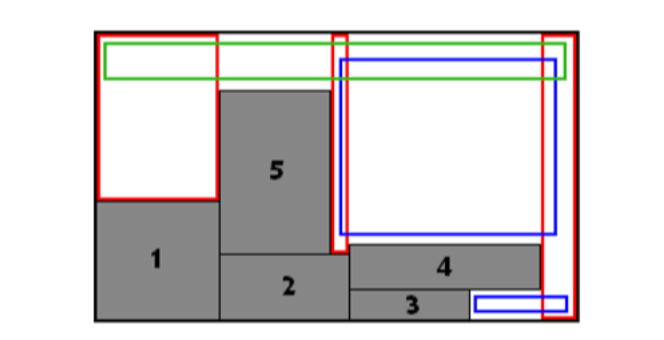
\includegraphics[width=0.8\textwidth]{packing/4.png}
    \caption{Пример упаковки алгоритмом максимальных прямоугольников \citep{Jylanki}}
    \label{fig:maxrects}
\end{figure}

Алгоритм максимальных прямоугольников по лучшей свободной области (Maximal Rectangles Best Area Fit (MAXRECTS-BAF)) позволяет использовать то же правило, которое было в аналогичном алгоритме гильотины. Мы выбираем $F_i \in S$, который наименьший в области, чтобы  разместить прямоугольник $R$ внутри. Если они равны, то используем  GUILLOTINE-BSSF.

Алгоритм максимальных прямоугольников по лучшей меньшей стороне (Maximal Rectangles Best Short Side Fit (MAXRECTSBSSF)) находит разницу между длинами сторон $R$ и $F_i$. Упаковывается $R$ в такой $F_i$, в котором $min(w_f – w, h_f – h)$ наименьший. Минимизируется длина меньшей стороны прямоугольника.

Алгоритм максимальных прямоугольников по лучшей большей стороне (Maximal Rectangles Best Long Side Fit (MAXRECTS-BLSF)). Упаковывается $R$ в такой $F_i$, в котором $max(w_f – w, h_f – h)$ наименьший. Минимизируется длина большей стороны прямоугольника.

Все алгоритмы могут быть реализованы за $O((|S|^2)*n)$ по времени и $\theta(|S|)$ по памяти, поэтому важно знать скорость роста $|S|$, чтобы вычислить фактическую сложность.

\section{Алгоритмы линии горизонта}

Алгоритм максимальных прямоугольников включал в себя трудоемкий процесс поддержки списка максимальных свободных прямоугольников, но можно использовать упрощенный алгоритм для реализации эвристики нижнего левого угла. Алгоритм линии горизонта работает с потерями, как и алгоритм выступа. Он не идеален в поиске свободных областей контейнера и может помечать некоторые неиспользованные области как использованные. Зато его процедура упаковки гораздо быстрее, чем в максимальных прямоугольниках.

Покажем использование алгоритма горизонта на примере города \citep{skyline}. Горизонт города - это внешний контур силуэта, образованного всеми зданиями в этом городе, если смотреть на него издалека. Теперь предположим, что даны местоположения и высота всех зданий. Необходимо найти горизонт, образованные силуэтом городских зданий.

Алгоритм линии горизонта работает, используя список «горизонтов» или крайних ребер, сформированный самыми верхними ребрами уже упакованных прямоугольников. Списком просто управлять, и он растет линейно вместе с количеством упакованных прямоугольников.

Алгоритм линии горизонта нижнего левого угла (Skyline Bottom-Left (SKYLINE-BL)) использует эвристику нижнего левого угла. Мы упаковываем прямоугольник $R$, выровненный по левому краю над уровнем горизонта, в результате чего верхняя сторона $R$ находится в самом нижнем положении. Так как $R$ можно повернуть, это может быть не уровень горизонта, находящийся в самой низкой позиции.

Алгоритм линии горизонта с лучшей вставкой (Skyline Best Fit (SKYLINE-BF)). Так как алгоритм линии горизонта иногда теряет информацию о свободных областях, нужно минимизировать потери. Для каждой позиции, куда можно упаковать прямоугольник, высчитывается общее пространство контейнера, которое будет потеряно, если поставить прямоугольник именно там. Затем выбирается позиция, которая минимизирует эту потерю. Если они равны, что использует правило нижнего левого угла, чтобы выбрать.

Алгоритмы линии горизонта реализуются за $O(n^2)$ по времени и $O(n)$ по памяти.

\section{Результаты тестов}

Производительность каждого алгоритма была исследована \citep{Jylanki}. Сгенерировав множество прямоугольников самых разных размеров, авторы получили следующие результаты (1.0 - алгоритм работает очень хорошо, но чем больше результат единицы, тем хуже): 

\begin{center}
\begin{tabular}{ c|c }
 Алгоритм & Средняя производительность \\
 \hline
  SHELF & 1.571 \\ 
  GUILLOTINE-MINAS-RM-BNF-BAF & 1.445 \\ 
  GUILLOTINE-LAS-RM-BNF-BSSF & 1.773 \\
  MAXRECTS-BSSF-BNF & 1.408 \\
  MAXRECTS-BSSF-BBF & 1.041 \\
  MAXRECTS-BSSF-BBF-GLOBAL & 1.005 \\
  MAXRECTS-BSSF-BBF-DESCSS & 1.009 \\
  SKYLINE-BL-WM-BNF & 1.392 \\
  SKYLINE-MWWM-BFF-DESCSS & 1.013 \\
\end{tabular}
\end{center}

\section{Пример реализации}

Так как наибольшую производительность показал алгоритм MAXRECTS-BSSF-BBF-GLOBAL, именно его реализация была выполнена. Алгоритм получает на вход размер корзины, произвольное количество прямоугольников, и выдает координаты внутри контейнера. Результатом стало следующее приложение, которое генерирует разные прямоугольники случайных размеров или создает прямоугольники с размерами, указанными заранее (рис. \ref{fig:maxrects-impl}) и заполняет ими предопределённый контейнер (рис. \ref{fig:maxrects-impl2}).
\newline
\newline
Исходный код приложения: \url{https://github.com/trszdev/maxrects-bssf-global-demo}
\newline
Демонстрация: \url{https://trszdev.github.io/maxrects-bssf-global-demo}

\begin{figure}
    \centerfloat
    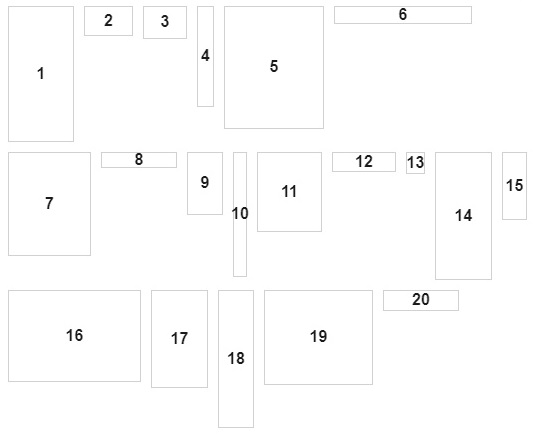
\includegraphics[width=0.6\textwidth]{packing/5.jpg}
    \caption{Тестовый набор прямоугольников для упаковки}
    \label{fig:maxrects-impl}
\end{figure}

\begin{figure}
    \centerfloat
    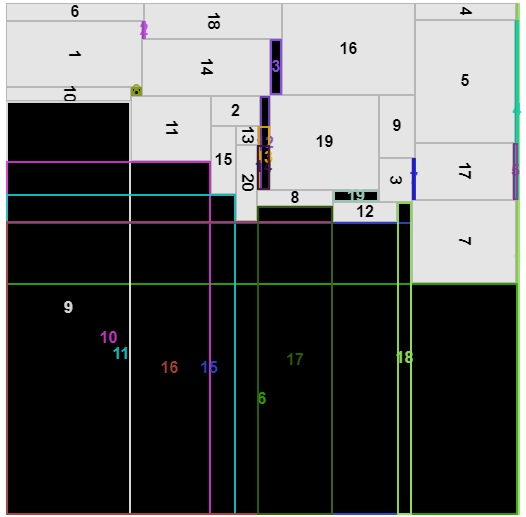
\includegraphics[width=0.6\textwidth]{packing/6.jpg}
    \caption{Контейнер, содержащий тестовый набор}
    \label{fig:maxrects-impl2}
\end{figure}

\chapter{Процедурная генерация уровней}

\parindent=1cm
Процедурная генерация позволяет создавать игровой уникальный контент, причем даже во время игры. Пусть стоит задача сгенерировать карту уровня, при том что карты на каждом уровне должны быть разными, но при этом связными и похожими на реальные помещения по своему расположению. Самым примитивным вариантом можно назвать генерацию случайных прямоугольников, когда пространство карты заполняется каким-то образом соединенными прямоугольниками, которые служат комнатами. Но если более сложные и эффективные варианты.

\section{Процедурная генерация уровней с помощью клеточных автоматов}

В семидесятых годах математик Джон Конвей опубликовал описание игры «Жизнь». Это не совсем настоящая игра, а скорее симулятор, который принимает на вход сетку, состоящую из клеток (живых или мертвых), и выполняет некоторые правила. Всего этих правил четыре:

1. Если у живой клетки меньше двух соседей (сосед — любая живая клетка из восьмисвязной области), она умирает.

2. Если у живой клетки есть два или три соседа, то она остается живой.

3. Если у живой клетки больше трех соседей, то она умирает.

4. Если у мертвой клетки есть в точности три соседа, то она оживает.

Если поэкспериментировать с различными комбинациями начальной сетки, то порой результат может получиться очень странным. Бесконечные циклы, фигуры, меняющие свою форму, и многое другое. Игра «Жизнь» — это пример клеточного автомата — сетки с клетками, чье поведение регулируется определенными правилами.

Для процедурной генерации уровня с помощью клеточного автомата необходимо реализовать нечто близкое к «Жизни», но чтобы на выходе получались не странные фигуры, а карта уровня \citep{cellar}.

Для этого создаем двумерный булевый массив, который будет иметь размеры карты. Значение «1» в ячейке будет означать живую клетку, значение «0»  — пустую. Заполнение значения происходит случайно для каждой ячейки, например, с коэффициентом 0,45. На выходе получается беспорядочная сетка с ячейками, которая вряд ли будет похожа карту уровня, а скорее напомнит qr-код. Однако это только инициализация исходной сетки, которую нужно «оживить» и заставить видоизменяться по заданным правилам.

Подобно игре «Жизнь» на каждом шаге каждая клетка будет проверяться на соответствие правилам и, вероятно, менять свое состояние. Посчитаем для клеток количество живых и мертвых соседей в восьмисвязной области. Правила гораздо более просты, чем для «Жизни» и выглядят так: заведем два значения «норма рождения» и «норма смерти» для оживления мертвых клеток и для убийства живых, соответственно. Если живые клетки окружены клетками в количестве меньшем, чем «норма смерти», то они умирают. Если мертвые клетки окружены клетками в количестве меньшем, чем «норма рождения», то они оживают.
Таким образом, итоговый результат будет зависеть от следующих величин:

- число, означающее насколько плотно изначальная сетка забита живыми клетками;

- нижняя граница количества соседей, начиная с которой клетки умирают;

- верхняя граница количества соседей, начиная с которой клетки умирают;

- количество соседей, которое оживляет мертвую клетку;

- количество итераций автомата.

Варьируя эти величины, можно получать разные результаты. Например, чем больше итераций автомата, тем менее беспорядочной будет итоговая сетка.

\begin{figure}
    \centerfloat
    
\includegraphics[width=0.5\textwidth]{levels/1.png}
    \caption{Пример работы клеточного автомата \citep{cellar}}
    \label{fig:cellular}
\end{figure}

Такой сетка становится уже после 6 итераций. У неё гладкий контур, она связная и вполне похожа на схему игрового уровня (рис. \ref{fig:cellular}).

\section{Процедурная генерации уровней с помощью BSP-деревьев}

BSP – binary space partitioning – двоичное разбиение пространства может применяться для генерации уровней. Нужна двумерная карта, которая будет схемой игрового уровня. Генерация происходит следующим образом: область разделяется на сегменты, в них создаются комнаты и соединяются коридорами \citep{bsp}.

Основой алгоритма будет служит класс Лист – область на карте, которая делится по вертикали или по горизонтали на два листа меньшего размера, и потом этот процесс повторяется с дочерними листьями, пока размер области после разделения не станет меньше либо равен некоторой константе, означающей минимальный возможный размер, меньше которой листья не нужны. Процедуру можно выполнять рекурсивно (рис. \ref{fig:bsp}). Алгоритм гарантирует, что Лист и содержащиеся в них комнаты будут распределяться по карте равномерно (за счет деления на два), а также между комнатами можно будет расположить коридоры (за счет того, что иерархия Лист связная).

\begin{figure}
    \centerfloat
    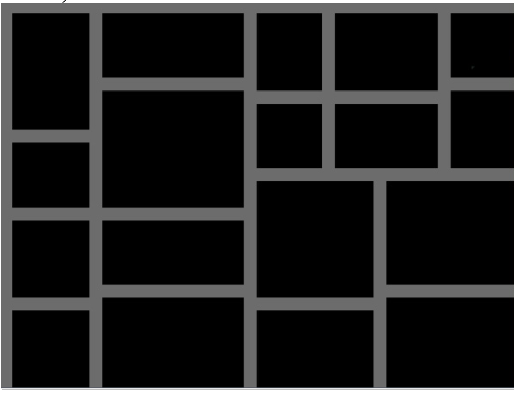
\includegraphics[width=0.6\textwidth]{levels/2.png}
    \caption{Разбиение карты на листья \citep{bsp}}
    \label{fig:bsp}
\end{figure}

По сути Лист это прямоугольная область. В каждом из Листов необходимо создать комнату. Размер и положение комнаты можно сгенерировать случайно, учитывая что размер должен быть меньше размера Листа, а расположить комнату можно в любом месте Листа, не выходя за его пределы (рис. \ref{fig:bsp2}). Таким образом, количество комнат равно количеству листьев. Они тоже распределены равномерно и тоже могут быть связаны коридорами.

\begin{figure}
    \centerfloat
    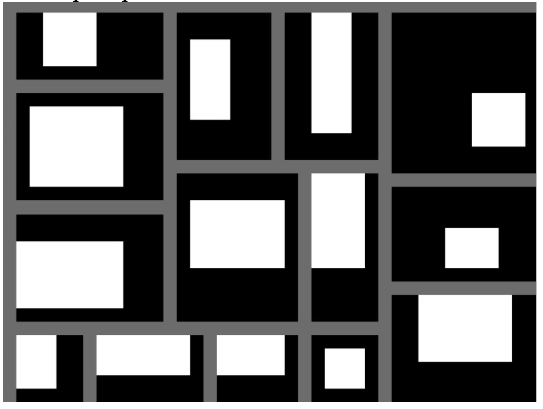
\includegraphics[width=0.6\textwidth]{levels/3.png}
    \caption{Создание комнат внутри листьев \citep{bsp}}
    \label{fig:bsp2}
\end{figure}

Коридоры — это связь дочерних листьев с родительскими. Рассмотрим лист, пройдем до его дочерних листьев, пока не наткнемся на комнату, а потом соединим комнаты. В комнатах, которые нужно соединить, выбираем случайные точки и соединяем их коридором заданной ширины (рис. \ref{fig:bsp3}).

\begin{figure}
    \centerfloat
    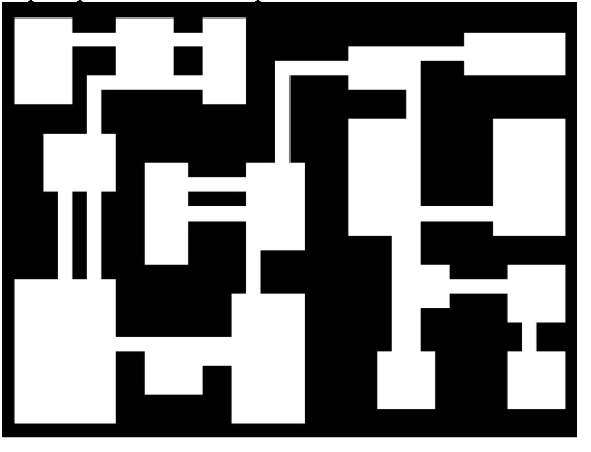
\includegraphics[width=0.6\textwidth]{levels/4.png}
    \caption{Соединение комнат коридорами \citep{bsp}}
    \label{fig:bsp3}
\end{figure}

Алгоритм гарантирует, что не останется изолированных комнат, так как все листья связаны друг с другом. Остается только модернизировать алгоритм, чтобы коридоры не могли располагаться слишком близко друг к другу.

\section{Процедурная генерации уровней с помощью туннелирования}

Туннелирование гарантирует, что карта уровня получится связной с большим количеством различных узких путей и незаполненного пространства. Для оптимальных результатов алгоритму требует карта с динамически изменяемым размером, иначе разметка уровня быстро выйдет за границу карты, и результат получится эстетически неудовлетворительным \citep{tunnel}.

Алгоритм действует следующим образом:

Пусть есть двумерный массив карты, где каждый элемент может принимать значение либо «стена» (по стене нельзя пройти), либо «пол» (по полу можно пройти).

1. Инициализируем карту, где каждая клетка — стена

2. Выбираем любую клетку карты как начальную точку

3. Превращаем выбранную клетку в пол

4. Пока недостаточное количество клеток было превращено в пол,

5. Делаем шаг в случайном направлении

6. Если новая клетка карты — стена, то превращаем её в пол и инкрементируем счетчик клеток, превращенных в пол

\section{Процедурная генерации уровней с помощью триангуляции Делоне}

Вначале на карте следует предварительно расположить объекты, которые будут использоваться во время игры: коридоры, двери, стены, комнаты. Можно сделать это «руками», если существует какой-нибудь план уровня, однако можно и раскидать по карте прямоугольники различных размеров. Естественно, они будут пересекаться и даже перекрывать друг друга, поэтому после генерации их следует разделить, либо с самого начала ставить условием генерации то, что они не должны пересекаться \citep{room}.

Следующим шагом надо определить, какие из комнат-прямоугольников будут основными/центральными. Для этого следует выбирать комнаты, которые находятся выше определенного порога ширины/высоты. Например, в качестве порога можно установить 1,25 * ((ширина + высота)/2). Если ширина и высота равны 24, то будут выбраны комнаты с шириной и высотой больше 30.

После этого с выбранными прямоугольниками проводим триангуляцию Делоне и получаем связный граф, состоящий из треугольников. У этого графа находим минимальное остовное дерево, в котором основные комнаты гарантированно достижимы, и при этом путей из одной комнаты в другую не так много. Это полезно, потому что нам не нужно полносвязная карта, и при этом в ней нет изолированных комнат. Однако карта с одним линейным путем — тоже не самый лучший вариант, поэтому 15\% ребер, убранных при поиске остовного дерева, можно вернуть обратно.

После  всего этого добавляем на карту коридоры. Для этого проходим по каждой вершине графа и соединяем коридором каждую, смежную с ней. Если вершины достаточно близки по горизонтали (близки координаты y), то соединяем их горизонтальной линией. Если близки по вертикали, то соединяем вертикальной. Если вершины имеют далекие координаты, как по x, так и по y, то соединяем их двумя линиями в форме L (рис. \ref{fig:room}). «Близость» высчитывается как расстояние двух центральных точек в смежных прямоугольниках.

Затем добавляем прямоугольники, которые не были выбраны, как основные. Те, которые близки к основным, можно соединить с ними, а те, которые попали на линию коридора, становятся частью коридора.

\begin{figure}
    \centerfloat
    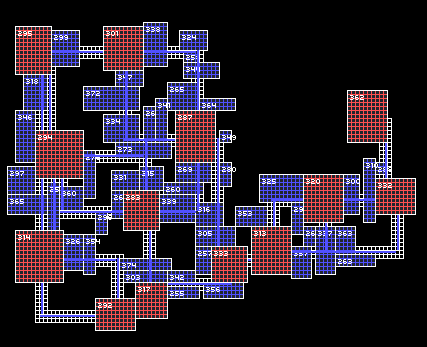
\includegraphics[width=0.6\textwidth]{levels/room.png}
    \caption{Прямые и L-образные коридоры \citep{room}}
    \label{fig:room}
\end{figure}

\section{Пример реализации}

Процедурная генерация уровней была выполнена с использованием BSP-деревьев. На вход алгоритм принимает размеры карты, глубину дерева, плотности комнат, врагов и сокровищ. Затем создается разряженное BSP дерево, вход и выход уровня располагаются по диаметру графа, а в комнатах размещаются монстры и сокровища с заданной плотностью. На выходе алгоритма получается клеточный уровень (рис. \ref{fig:bsp-impl} и \ref{fig:bsp-impl2}).
\newline
\newline
Исходный код приложения: \url{https://github.com/trszdev/bsp-level-generation-demo}
\newline
Демонстрация: \url{https://trszdev.github.io/bsp-level-generation-demo}

\begin{figure}
    \centerfloat
    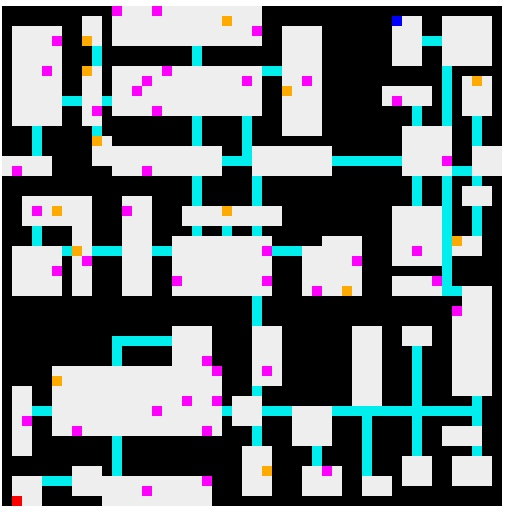
\includegraphics[width=0.45\textwidth]{levels/5.jpg}
    \caption{Уровень с высокой плотностью комнат}
    \label{fig:bsp-impl}
\end{figure}

\begin{figure}
    \centerfloat
    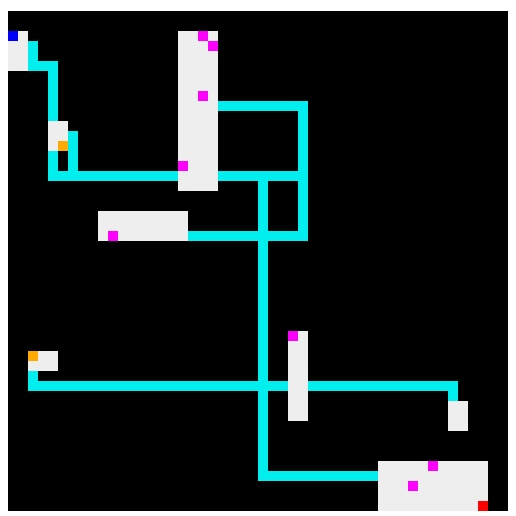
\includegraphics[width=0.45\textwidth]{levels/6.jpg}
    \caption{Уровень с низкой плотностью комнат}
    \label{fig:bsp-impl2}
\end{figure}

\chapter{Генерация пиксель-арта}

\parindent=1cm
Алгоритм генерации пиксель-арта из изображения в высоком разрешении с большой цветовой палитрой базируется на двух техниках \citep{pixel}.

\section{Простая линейная итеративная кластеризация (Simple Linear Iterative Clustering, SLIC)}

Этот метод разделяет изображение на области, называемые «суперпикселями». Он аналогичен методу кластеризации k-средних в пятимерном пространстве (в котором три цветовых и две позиционных координаты). Пиксели исходного изображения $p_$i присваиваются суперпикселям $p_s$ минимизацией

\begin{equation}
d(p_i, p_s) = d_c(p_i, p_s) + m \sqrt{\frac{N}{M}}d_p(p_i, p_s),
\end{equation}

где $d_c$ – разность между цветами, $d_p$ – разность координат, $М$ – количество пикселей исходного изображения, $N$ – количество суперпикселей и $m$ – значение из промежутка [0, 20], которое контролирует плотность цветов в итоговом изображении. Разность между цветами и координатами находится как евклидово расстояние, а цвета представлены в цветовом пространстве LAB. Пока происходит итерирование, суперпиксели приобретают цвет и позицию, соответствующие среднему значению исходных пикселей (рис. \ref{fig:slic}).

\begin{figure}
    \centerfloat
    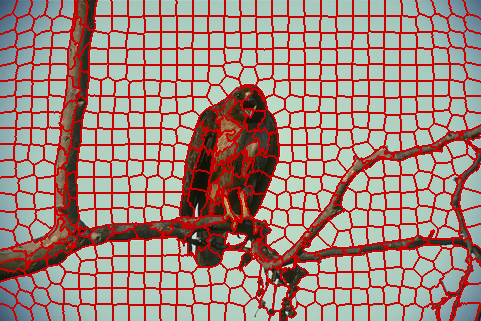
\includegraphics[width=0.6\textwidth]{pixel/slic.png}
    \caption{Пример работы алгоритма SLIC \citep{slic}}
    \label{fig:slic}
\end{figure}

\section{Ограниченный по массе детерминированный отжиг (Mass Constrained Deterministic Annealing, MCDA)}

Это глобальный метод оптимизации аналогичный процессу нормализации физического материала. Он используется для определения цветов в палитре и для нахождения соответствия каждого пикселя цвету из этой палитры.

Этот алгоритм основан на алгоритме кластеризации, который вероятностно присваивает объекты кластерам на основе их расстояния от каждого кластера. Он основан на температурном значении Т, которое рассматривается пропорционально ожидаемой дисперсии кластеров. Вначале T устанавливается в максимальное значение $T_0$, что делает каждый объект одинаково вероятно принадлежащим к любому кластеру. Каждый раз, когда система локально сходится в одной точке, $Т$ понижается, и дисперсия каждого кластера уменьшается. Когда это происходит, объекты начинают отдавать предпочтение конкретным кластерам, и когда $Т$ приближается к нулю, каждый объект эффективно присваивается одному кластеру, и создается окончательный набор кластеров (рис. \ref{fig:da}). Так как при высокой $Т$ наличие нескольких кластеров является избыточны, алгоритм начинает с одного кластера, представленного внутри двумя подкластерами. В начале каждой итерации эти подкластеры установлены с небольшими перестановками их средних значений. При высокой $Т$ эти кластеры сходятся к одному и тому же значению после нескольких итераций, но, когда температура снижается, они начинают естественным образом разделяться. Когда это происходит, кластер уже разделен на два кластера (представленных подкластерами). Деление происходит рекурсивно, пока максимальное число кластеров, установленное пользователем, не будет достигнуто.

\begin{figure}
    \centerfloat
    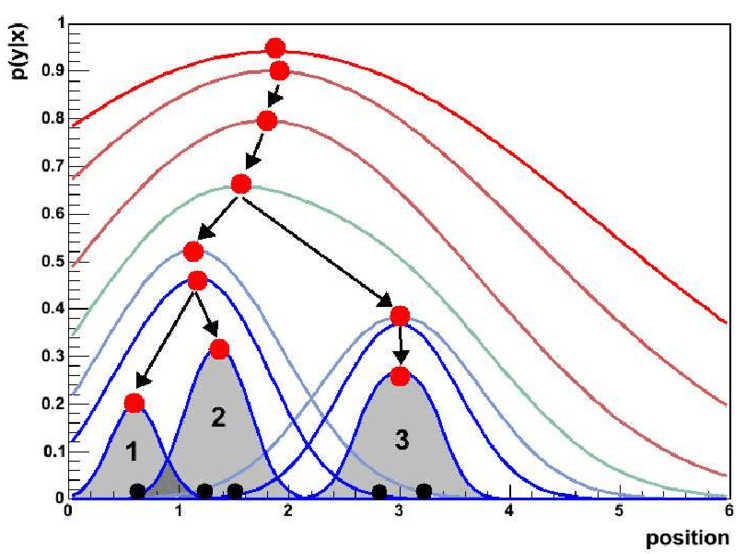
\includegraphics[width=0.6\textwidth]{pixel/da.png}
    \caption{Детерминированный отжиг \citep{da}}
    \label{fig:da}
\end{figure}

\section{Метод генерации}

Алгоритм работает итеративно, в его описании используются следующие термины:

- \textit{входные пиксели} – набор пикселей исходного изображения, обозначаемых $p_i$, где $i$ – число от 1 до $M$, где $M$ – площадь исходного изображения; 

- \textit{выходные пиксели} – набор пикселей получившегося изображения, обозначаемых $p_o$, где $o$ – число от 1 до $N$, где $N$ – площадь получившегося изображения; 

- \textit{суперпиксель} – область исходного изображения, обозначаемая $p_s$, где $s$ – число от 1 до $N$. Суперпиксели - это разделение исходного изображения;

- \textit{палитра} – набор из $K$ цветов $c_k$, $k$ – число от 1 до $K$ в цветовом пространстве LAB.

В общем виде алгоритм выглядит так:

1)  \textit{Инициализируются} суперпиксели, палитра и температура $T$

2)  Пока $T > T_f$

3)      \textit{Обработаем} суперпиксели с 1 шагом модифицированного алгоритма SLIC

4)      \textit{Соотнесем} суперпиксели с цветами палитры

5)      \textit{Обработаем} цвета в палитре

6)      Если палитра сводится в одну точку

7)          Уменьшим температуру $T = a*T$

8)          \textit{Расширим} палитру

9)  Выполним пост-обработку

\subsection{Инициализация}

$N$ центров суперпикселей инициализируются как сетка, наложенная на исходное изображение, и каждый входной пиксель назначается ближайшему суперпикселю. Палитра инициализируется одним цветом, для которого установлено среднее значение из $M$ входных пикселей. Всем суперпикселям присваивается этот средний цвет.

Температура $T$ установлена в $1,1*T_c$, где $Т_с$ – критическая температура набора входных $M$ пикселей, определяемая как двойная дисперсия вдоль главного компонента оси пространства LAB. $T_c$ набора объектов, назначенных кластеру, это температура, при которой кластер естественным образом разделится. Поэтому важно, чтобы начальная температура была немного выше температуры, при которой будет существовать больше одного цвета в палитре.

\subsection{Обработка суперпикселей}

Этот шаг алгоритма соотносит пиксели исходного изображения с суперпикселями. Для этого используется SLIC. В исходном алгоритме при каждой итерации входной пиксель соотносился с суперпикселем, который минимизировал $d(p_i, p_s)$, и цвет каждого суперпикселя устанавливался как средний цвет, связанных с ним входных пикселей $m_s$. Однако алгоритм следует модифицировать, чтобы цвет каждого суперпикселя устанавливался равным цвету палитры, связанной с этим суперпикселем. Эта взаимозависимость с палитрой оптимизирует суперпиксели по отношению к цветам в палитре, а не к цветам исходного изображения.

Затем следует выполнить два шага, один из которых модифицирует каждую координату $(x, y)$ суперпикселя для следующей итерации, а другой изменяет каждый цвет, представляемый суперпикселем.

Для первого шага используем сглаживание Лапласа. Каждый центр суперпикселя перемещается на определенный процент от расстояния от его текущего положения к среднему положению своих соседей из 4-связной области. Можно использовать значение 40\%.

Для второго шага цвета, представляемые суперпикселями, сглаживаются. В оригинальном SLIC представитель цвета каждого суперпикселя это средний цвет входных пикселей, входящих в этот суперпиксель. Однако простое использование среднего цвета может стать проблемой для градиентных областей. Избежать её помогает двусторонний фильтр. Мы строим изображение нужного размера (размера выходного изображения), где каждому суперпикселю присваивается та же позиция, что и выходному пикселю $m_s$. Цвета, которые вытекают из двусторонней фильтрации этого изображения $m_s’$, используются при итерации палитры.

\subsection{Работа с палитрой}

Итерация по палитре нарушается тремя этапами: соотнесением суперпикселей с цветами палитры, обработкой и расширением. Соотнесение и обработка встречаются на каждой итерации, а расширение происходит, когда палитра сходится для текущей температуры $T.$ Каждый подкластер рассматривается как отдельный цвет в палитре. Цвет $c_k$ – средний цвет двух его подкластеров. Когда палитра достигает максимального размера по количеству цветов, подкластеры исключают, и каждый цвет в палитре представляется единым кластером.

\subsection{Соотнесение}

Алгоритм MCDA требует вероятностную модель, которая указывает, насколько вероятно, что конкретный суперпиксель будет связан с каждым цветом в палитре. Условная вероятность $P(c_k|p_s)$ для суперпикселя $p_s$, которому назначен цвет $c_k$, зависит от расстояния в пространстве LAB и текущей температуры и вычисляется как

\begin{equation}
P(c_k|p_s) \propto P(c_k) e^{-\frac{||m_s' - c_k||}{T}}
\label{prob}
\end{equation}

$P(c_k)$ — вероятность того, что цвет $c_k$ соотносится с любым суперпикселем. После инициализации есть только 1 цвет, поэтому значение инициализируется в 1. Когда в палитру введено больше цветов, эта вероятность считается как 

\begin{equation}
P(c_k) = \sum_{s=1}^{N}P(c_k|p_s)P(p_s)
\end{equation}

В настоящий момент $P(p_s)$ имеет равномерное распределение. Значения $P(c_k)$ обновляются после вычисления $P(c_k|p_s)$. Каждому суперпикселю присваивается такой цвет в палитре, который максимизирует $P(c_k|p_s)$. Экспоненциальное распределение в уравнении (\ref{prob}) стремится к равномерному распределению про больших $T$, и в этом случае каждый суперпиксель будет равномерно связан с каждым цветом палитры. Когда $T$ уменьшается, суперпиксели выбирают те цвета палитры, до которых меньше расстояние. При конечной температуре $P(c_k|p_s) = 1$ для одного цвета в палитре и $P(c_k|p_s) = 0$ для остальных.

\subsection{Обработка}

Следующий шаг — это обработка палитры путем переназначения каждого цвета $c_k$ на средневзвешенное значение всех цветов суперпикселей, используя вероятность ассоциации с этим цветом

\begin{equation}
c_k = \frac{\sum_{s=1}^{N}m_s'P(c_k|p_s)P(p_s)}{P(c_k)}
\end{equation}

Эта формула адаптирует цвета в существующей палитре, учитывая пересмотренные суперпиксели. 

\subsection{Расширение}

Расширение происходит только во время итерации, если палитра сходится для текущей температуры $T$ (сходимость измеряется по общему изменению палитры с того момента, как последняя итерация была меньше, чем какое-то значение, принадлежащее палитре). Вначале температура снижается на коэффициент $a$ (например, 0.7). Затем палитра расширяется, если в ней меньше цветов, чем указал пользователь. Для каждого $c_k$ проверяется, нужно ли разделить цвет на два отдельных цвета в палитре. Согласно MCDA, каждый цвет в палитре представлен двумя точками кластера $c_k_1$ и $c_k_2$. Используем $\| c_k_1 - c_k_2 \| < \varepsilon$ (где $\varepsilon$ достаточно маленькое число), чтобы проверить разделение палитры. Если это так, то две точки кластера добавляются в палитру как отдельные цвета, каждый со своей парой кластерных точек.
После разрешения любых расщеплений, каждый цвет представлен двумя подкластерами с одинаковым значением (если не указано максимальное количество цветов, которое было достигнуто). Для того, чтобы любые подкластеры любого цвета были отделены в следующих итерациях,  $c_k_1$ и $c_k_2$ должны быть сделаны очень разными. Для этого нужно отклонить подкластеры каждого цвета на небольшое значение вдоль оси главного компонента кластера в пространстве LAB. Это отклонение позволяет подкластерам каждого цвета слиться, если $T > T_c$, иначе разделиться.

\section{Пример реализации}

Генерация пиксель-арта была выполнена двумя способами. Первый способ использует масштабирование по принципу ближайшего соседа и квантизацию цвета методом k средних. Второй способ представлен ранее. На вход алгоритм получает изображение, количество цветов в новой палитре и размер пикселя. На выходе получается новое изображение в стиле пиксель-арт (рис. \ref{fig:pixel-impl} и \ref{fig:pixel-impl2}).
\newline
\newline
Исходный код приложения: \url{https://github.com/trszdev/pixelart-generation}
\newline
Демонстрация: \url{https://trszdev.github.io/pixelart-generation}

\begin{figure}
    \centerfloat
    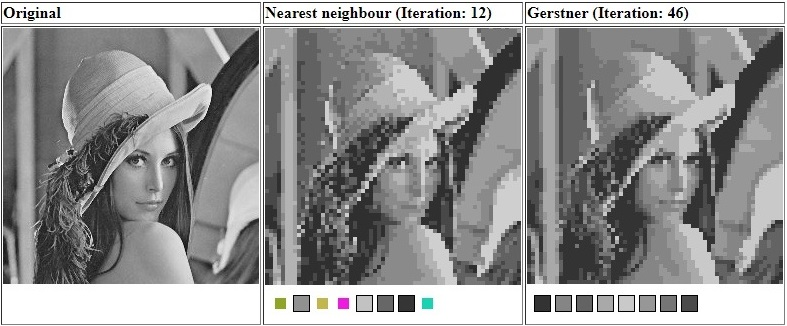
\includegraphics[width=0.85\textwidth]{pixel/2.jpg}
    \caption{Фотография Лены Сёдерберг. Количество цветов - 8, размер пикселя - 4}
    \label{fig:pixel-impl}
\end{figure}

\begin{figure}
    \centerfloat
    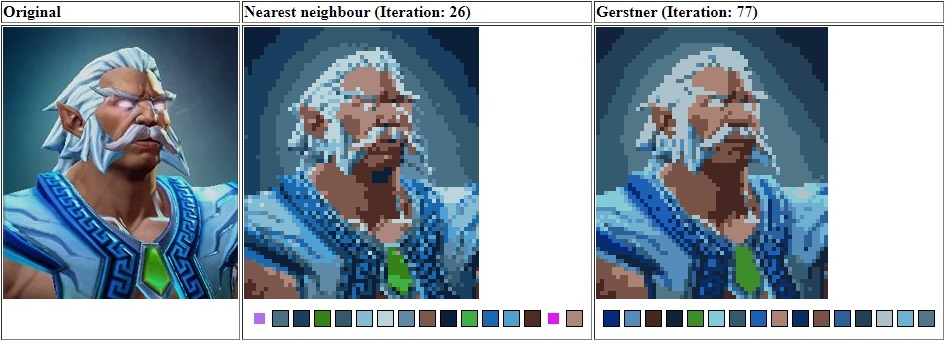
\includegraphics[width=1\textwidth]{pixel/3.jpg}
    \caption{Zeus - DotA 2. Количество цветов - 16, размер пикселя - 4}
    \label{fig:pixel-impl2}
\end{figure}

\chapter{Заключение}

\parindent=1cm
В результате проделанной работы поставленные задачи были тщательно проанализированы и решены алгоритмическим путём; приложения, реализующие конкретные алгоритмы размещены в открытом доступе в Интернете.

Несмотря на то, что итоговые решения достаточно хорошо справляются со своими задачами, в них присутствуют недостатки, исправление которых остаётся за рамками данной работы.

\section{Недостатки алгоритмов}
\subsection{MAXRECTS-BSSF-GLOBAL}
Синтетические тесты показали, что в среднем данный метод лучше всего упаковывает прямоугольники, но он никак не адаптируется к проблеме формирования атласа: нередки случаи, когда размер атласа значительно превышает упакованную область. В таком случае MAXRECTS-BSSF-GLOBAL проделает много лишней работы. Для решения этой проблемы предлагается использовать метод максимальных прямоугольников в связке с генетическим алгоритмом.

\subsection{Генерация уровня с помощью BSP}
Данный метод создает уровни с интересными коридорами: они получаются ветвистыми, иногда параллельными, иногда широкими. Однако, комнаты остаются неприметными прямоугольниками. Для решения этой проблемы предлагается использовать клеточный автомат на комнатах и/или использовать заранее заготовленные участки карт.

\subsection{Пикселизация методом Герстнера}
Несмотря на заметный прогресс по сравнению с наивным методом, данный алгоритм нуждается в изображениях, содержащих малое количество деталей. Помимо этого, кластеризация суперпикселей порой игнорирует пиксельные примитивы линий, из-за чего те получаются неровными и некрасивыми; кластеризация цвета "теряет"\ редкие цвета (например, цвет глаз). 

\bibliographystyle{plainurl}
\bibliography{references}
\end{document}
